\section{Hindcast Results}
	\subsection{Model Evaluation}
		Table \ref{tab:results-evaluation-inside-mm} shows the evaluation results for the three cities inside Metro Manila: Manila, Pasay, and Quezon.
		All MB and RMSE values fall within the recommended values of $\leq \pm \qty{2.0}{\degreeCelsius}$ and $\leq \qty{3.5}{\degreeCelsius}$, respectively.
		This shows that these simulations correctly follow the average air temperature for these respective cities.
		Despite this, many runs show an IOA value $< 0.8$, indicating that these runs show bad agreement between the simulation and observed data.
		While these runs may follow the average trend for air temperature in these cities, it may not be capturing the details of how the temperature changes.
		
		\begin{table}[]
			\caption{Evaluation results for the three cities inside Metro Manila. Values that do not match the recommended values are colored in red.}
			\label{tab:results-evaluation-inside-mm}
			\centering
			\begin{tabular}{lrSSSS}
				\hline \hline
				ICBC     & \multicolumn{1}{c}{ds [\unit{km}]} & {MB [\unit{\degreeCelsius}]} & {MAE [\unit{\degreeCelsius}]}                          & {RMSE [\unit{\degreeCelsius}]} & {IOA}                               \\
				\hline
				\multicolumn{6}{c}{\textit{Manila}}                                                                                                  \\
				EIN15    & 16                          & -0.53   & 1.27                              & 1.61      & \color{red} 0.78 \\
				EIN15    & 8                           & 0.90    & 1.45                              & 1.84      & 0.85                              \\
				CNRM-CM5 & 16                          & -0.73   & 1.63                              & 2.09      & \color{red}0.57 \\
				CNRM-CM5 & 8                           & -0.38   & 1.87                              & 2.33      & \color{red}0.75 \\
				\multicolumn{6}{c}{\textit{Pasay}}                                                               \\
				EIN15    & 16                          & -0.59   & 1.24                              & 1.55      & 0.88                              \\
				EIN15    & 8                           & 0.94    & 1.40                              & 1.75      & 0.88                              \\
				CNRM-CM5 & 16                          & -0.72   & 1.87                              & 2.39      & \color{red} 0.52 \\
				CNRM-CM5 & 8                           & -0.37   & 1.78                              & 2.22      & \color{red} 0.79 \\
				\multicolumn{6}{c}{\textit{Quezon}}                                                                                  \\
				EIN15    & 16                          & -0.61   & 1.45                              & 1.81      & 0.88                              \\
				EIN15    & 8                           & 0.57    & 1.33                              & 1.70      & 0.91                              \\
				CNRM-CM5 & 16                          & -0.10   & \color{red} 2.29 & 2.77      & \color{red} 0.46 \\
				CNRM-CM5 & 8                           & -0.75   & 1.95                              & 2.44      & 0.81  \\                           
				\hline
			\end{tabular}
		\end{table}
		
		For the MAE, the CNRM-CM5 run with 16 km horizontal resolution has a value of $2.29$ in Quezon, which does not fall within the recommended value of $\leq \pm \qty{2.0}{\degreeCelsius}$.
		All other MAE values for runs in Manila, Pasay, and Quezon fall within the recommended value.
		The same run also exhibits the lowest IOA value of $0.46$, indicating that this run exhibits the poorest agreement between the simulation and observed data.
		A graph of the simulation data and observed data for Quezon using CNRM-CM5 can be seen in Figure \ref{fig:cnrm-sim-vs-observed-quezon}. 
		The simulation with the lower grid cell resolution was able to follow the average trend of the observed data, but its oscillations were much smaller than the observed data.
		The simulation with the finer resolution matches the large oscillations of the observed data more closely (Figure 2b).
		This may indicate that the high MAE is due to the failure of that run to replicate the oscillations of the observed data.
		More graphs comparing the simulated and observed data for Manila, Quezon, and Pasay are found in Appendix \ref{app:model-evaluation-graphs}.

		
		\begin{figure}	
			\centering
			\includegraphics[width = \textwidth]{CNRM 16 km/Quezon}
			\includegraphics[width = \textwidth]{CNRM 8 km/Quezon}
			\caption{
				A comparison of the simulated data (orange) and observed data (blue) in the city of Quezon using the CNRM-CM5 ICBC with 16 km resolution (above) and 8 km resolution (below).
			}
			\label{fig:cnrm-sim-vs-observed-quezon}
		\end{figure}
		
		Table \ref{tab:results-evaluation-outside-mm} shows the evaluation results for the three cities outside of Metro Manila: Baguio, Angeles, and Olongapo.
		For Baguio, three out of the four sensitivity runs performed poorly.
		The EIN15 run with 16 km resolution exhibited MB, MAE, and IOA values outside of the recommended value.
		The CNRM-CM5 run with 16 km resolution had all of its performance statistics fall outside of the recommended values, and showed the lowest IOA out of all the cities and runs.
		While the MB and RMSE of the CNRM-CM5 run with 8 km resolution are within recommended values, its MAE and IOA do not.
		Only the EIN15 run with 8 km resolution show all performance statistics within recommended values.
		A graph of the observed data and simulation data using CNRM-CM5 for Baguio is seen in Figure \ref{fig:cnrm-sim-vs-observed-baguio}.
		The lower resolution run overshoots the observed data by around $\qty{8}{\degreeCelsius}$, and exhibits smaller oscillating behavior compared to the observed data.
		The higher resolution shows a closer match to the observed data, with the simulation roughly matching the trend and oscillating behavior of the observed.
			
		\begin{table}[]
			\caption{Evaluation results for the three cities inside Metro Manila. Values that do not match the recommended values are colored in red.}
			\label{tab:results-evaluation-outside-mm}
			\centering
			\begin{tabular}{lrSSSS}
				\hline \hline
				ICBC     & \multicolumn{1}{c}{ds [\unit{km}]} & {MB [\unit{\degreeCelsius}]} & {MAE [\unit{\degreeCelsius}]}                          & {RMSE [\unit{\degreeCelsius}]} & {IOA}                               \\
				\hline
				\multicolumn{6}{c}{\textit{Baguio}}                                                                                                                                                    \\
				EIN15    & 16                          & \color{red} 2.48 & \color{red}  2.60  & 3.08                              & \color{red}  0.76  \\
				EIN15    & 8                           & 1.49                              & 1.91                              & 2.33                              & 0.84                              \\
				CNRM-CM5 & 16                          & \color{red}  8.77  & \color{red}  8.77  & \color{red}  9.10  & \color{red}  0.32  \\
				CNRM-CM5 & 8                           & 0.60                              & \color{red}  2.05  & 2.62                              & \color{red}  0.79  \\
				\multicolumn{6}{c}{\textit{Angeles}}                                                                                                                      \\
				EIN15    & 16                          & -0.48                             & 1.47                              & 1.83                              & 0.90                              \\
				EIN15    & 8                           & -0.64                             & 1.48                              & 1.87                              & 0.91                              \\
				CNRM-CM5 & 16                          & 0.41                              & \color{red}  2.42  & 2.84                              & \color{red}  0.45  \\
				CNRM-CM5 & 8                           & -1.98                             & \color{red}  2.59  & 3.13                              & \color{red}  0.76  \\
				\multicolumn{6}{c}{\textit{Olongapo}}                                                                                                                                      \\
				EIN15    & 16                          & -1.52                             & 1.80                              & 2.16                              & 0.85                              \\
				EIN15    & 8                           & -0.55                             & 1.55                              & 1.95                              & \color{red}  0.78  \\
				CNRM-CM5 & 16                          & 0.06                              & \color{red}  2.18  & 2.63                              & \color{red}  0.44  \\
				CNRM-CM5 & 8                           & -1.21                             & 1.98                              & 2.51                              & \color{red}  0.67 \\
				\hline
			\end{tabular}
		\end{table}
		
		\begin{figure}	
			\centering
			\includegraphics[width = \textwidth]{CNRM 16 km/Baguio}
			\includegraphics[width = \textwidth]{CNRM 8 km/Baguio}
			\caption{
				A comparison of the simulated data (orange) and observed data (blue) in the city of Baguio using CNRM-CM5 with 16 km resolution (above) and 8 km resolution (below).
			}
			\label{fig:cnrm-sim-vs-observed-baguio}
		\end{figure}
		
		From these results, Baguio is shown to be hard to accurately simulate.
		One reason why this may be the case is because of the topology of the city.
		Baguio's elevation is about 1,500 m above sea level, unlike the other cities which are situated near sea level.
		Furthermore, since Baguio is situated on a mountain, its nearby topology is sloped, unlike other cities where it is mostly level.
		This more complex topology may need a higher resolution in order to accurately simulate the atmospheric conditions of that region.
		
		For Angeles, the two EIN15 runs have evaluation statistics that match the recommended values.
		Furthermore, the two runs show the highest IOA values among all the runs, with a value of $0.90$ for the 16 km run and $0.91$ for the 8 km run.
		The two CNRM-CM5 runs in Angeles both have MB and RMSE values that pass the benchmark, but have MAE and IOA values that do not.
		
		For Olongapo, the two EIN15 runs both show good results among all the metrics, except for the IOA.
		The two CNRM-CM5 runs also show a low IOA, indicating inaccurate values for this station.
		
		It can be seen that in general, increasing the horizontal resolution of the simulation will increase the IOA, giving a more accurate simulation.
		One exception to this observation is for Olongapo.
		When going from a 16 km resolution to an 8 km resolution using EIN15, MB, MAE, and RMSE values improved, but the IOA worsened from $0.85$ to $0.78$.
		A graph of the observed data and simulation data using EIN15 for Olongapo is seen in Figure \ref{fig:ein15-sim-vs-observed-olongapo}.
		While the simulation using the lower resolution undershoots the observed temperature by a few degrees Celcius, the size of its oscillations closely resemble the observed data.
		The simulation using the higher resolution exhibits a smaller oscillation size compared to the observed data, though its average more closely follows the observed.
		One reason for this may be because of the station being situated by a bay.
		The nearby water can play a part with the station’s air temperature, which the simulation settings may not have accounted for.
		With the lower resolution, the interaction with water may have been negligible enough as to not affect settings, but the higher resolution gives more grid cells over water, which is perhaps why the accuracy worsened.		
		
		\begin{figure}	
			\centering
			\includegraphics[width = 0.8 \textwidth]{EIN15 16 km/Olongapo}
			\includegraphics[width = 0.8 \textwidth]{EIN15 8 km/Olongapo}
			\caption{
				A comparison of the simulated data (orange) and observed data (blue) in the city of Olongapo using EIN15 with 16 km resolution (above) and 8 km resolution (below).
			}
			\label{fig:ein15-sim-vs-observed-olongapo}
		\end{figure}
		
		Out of the four runs, the run using EIN15 with 8 km resolution performs the best.
		The IOA values for each station, except Olongapo, matches the recommended values of $> 0.8$.
		This means that simulations using these settings are accurate for the places studied, and can be used for future research.
		One limitation of EIN15 is that it is not compatible for forecasts, only hindcasts. Studies of future trends will need to use another ICBC such as CNRM-CM5, which is  a general climate model that does support forecasting.
		One trade-off though in using a higher horizontal resolution is that it can slow down the time it takes for the simulation to finish, as the simulation needs more grid cells.
		Also, for a given horizontal resolution, the EIN15 run performed more accurately compared to the CNRM-CM5 run. 
		This shows that runs using CNRM-CM5 need a higher horizontal resolution than EIN15 in order to exhibit the same accuracy.
		
		One limitation of this study is that it only studies one variable, namely: near-surface air temperature.
		It does not examine ground temperature or temperature at different elevations.
		It also does not examine other factors that may be relevant to the study of urban heat islands, such as humidity, wind speed, wind direction, or precipitation. 
		Another limitation is that this study only examines the three-year period from 2015 to 2017.
		Future studies may choose to study these other variables or study longer timeframes.
		
		There are many factors that can affect the findings. 
		Firstly, the physics schemes used in this run are all the default schemes, with the exception of the Community Land Model version 4.5 being chosen over the default BATS1e. 
		These runs do not use other models such as a lake model or a chemistry model, which may make the simulations more accurate and is an avenue for future research.
		Next, simulations are compared to the weather station data from the ISD.
		Only six stations were considered in this study.
		The data will be as accurate as the instruments used to record the data.
		Lastly, the study only used one domain.
		Changing the size and location of the domain without tweaking other settings can change the accuracy of the simulation.
		
		
		
		
		
		